\documentclass[UTF8]{ctexart}
\pagestyle{plain}
\usepackage{amsmath}
\usepackage{geometry}
\geometry{a4paper,scale=0.7}
\usepackage{enumitem}
\setlist[description]{leftmargin=\parindent,labelindent=\parindent}
\usepackage{graphicx}
\usepackage{float}
\usepackage{subfigure}
\title{文本分类算法综述}
\author{罗伟斌}
\begin{document}
\maketitle
\section{简介}
	在当今信息爆炸的世界,我们可以接触到海量各种各样的数据和信息,包括文本、声音、图像等,而在这海量信息中大部分的都是以文本(Text)方式存在的,比如,电子文档,电子邮件等。海量的信息同样也带来了信息杂乱的烦恼,为了快速、准确地找到我们所需要的信息,我们就必须对这些文本进行有效的管理和组织,挖掘蕴藏在其中的文本信息。文本分类技术作为一个能有效管理和发掘文本信息的技术,在过去的几十年中得到了蓬勃的发展,并且已经在信息检索、医疗诊断、新闻分类、搜索引擎等众多领域得到了广泛的应用。

\subsection{文本分类问题定义}
	\par 文本分类问题可以定义为如下:将布尔值(Boolean)赋予属于集合$D×C$中的每一对记录$<d_j , c_i>$,D表示文本的集合,$C=\{c_1 , c_2 , c_3 ,\ldots , c_{|C|}\}$是预定义类标签值的集合。若项$<d_j, c_i>$被赋予布尔值T则表示文本$d_j$的类标签为$c_i$, 若项$<d_j,c_i>$被赋予布尔值为F,则代表文本$d_j$的类标签不为$c_i$。简而言之,文本分类任务就是找出未知函数$\tilde{\Phi}:D×C\to\{T,F\}$,使得$\tilde{\Phi}$尽可能的近似于或接近于目标函数函数$\Phi$,$\tilde{\Phi}$被称为分类器,也叫假设或者模型。我们假定在文本分类任务中已满足如下条件,类标签值为符号值,并不包含额外含义。除了文本本身内容之外,不包含文本类型,发布日期等外在信息。

\subsection{单标签与多标签文本分类}
	\par 在不同的应用场景中,可能会对文本分类任务加入额外的约束条件,比如限定对于$d_j\in D$只能有确定的K个标签值,其中当K为1时,被称之为单标签分类(single-label classification), 对于每个$d_j\in D$, K可以为0到$|C|$时,称之为多标签分类(multilabel classification)。单标签分类中有个特殊情况是二分类,则意味着$d_j\in D$要么标签值为ci要么为$\overline{c_i}$。
	\par 多标签分类问题可以转化为多个二分类问题,只需要将在标签集合$C=\{c_1,\ldots, c_{|C|}\}$下的多标签分类分解为$\vert C \vert$个独立的在标签集合$\{c_i, \tilde{c_i} \}$(i=1, ......, $\vert C \vert$)二分类问题。当然上面的转换必须保证上述标签集中必须是统计意义上两两相互独立的,对于任意的$c'$, $c''$, $\tilde{\Phi}(d_j, c')$
	与$\tilde{\Phi}(d_j, c')$相互独立。这也就意味着当符合上述条件时,对于单标签文本分类问题的算法可以使用与多标签文本分类问题,但是反过来一般是不成立的。

\subsection{文本分类的应用与方法}
    \par 文本分类技术已经在文本挖掘的多个领域得到了广泛的应用,以下介绍几个最典型的应用场景:
    \begin{description}
    	\item[新闻分类与管理] 现今新闻机构每天都会产生大量的新闻稿件,以至于新闻服务机构(如新闻门户网站)通过无法通过人工有效管理和分门别类,因此文本分类技术在新闻分类方面被广泛应用也就不足为奇了。 
    	\item[文档管理与查询] 除了新闻服务机构,需要处理大量文本文档的地方都有文本分类技术的用武之地,比如在大型的电子图书馆,互联网存档机构和科技著作管理机构等这些地方,对文档良好的层次化管理对查询效率有很大的帮助。
    	\item[情感分析] 微博,论坛,购物网站等等类似的网站都会有大量的用户数据生成,对用户或顾客的反馈或评价进行整理和分析,了解用户的观点,态度,情感倾向等,可以得有用的具有指导性信息。
    	\item[垃圾邮件检测] 像Google或微软等公司都在其邮箱应用中使用文本分类技术来加强对垃圾邮件的过滤,以便向用户提供更好的服务。
    \end{description}
	\par 由于文本分类本身是一个分类问题,因此一般的模式分类方法都可以应用于文本分类的研究。但是在介绍这些算法之前,首先应该了解的如何获取各种文本特征,各种特征应该赋予多大的权值,已经有多种可以表征文本特征的方法,这其中包括了基于文档频率(document frequency)的特征提取,基尼系数(gini-index),信息增益(information gain),$\chi^2$统计量和互信息(mutual information)等方法。通过这些方法可以获得文本的多方面特征,有了这些特征,可以将文本表示成空间向量形式(vector space),近年来的研究是以词嵌入(word embedding)来表征词,进而构建对文本的表示形式。对不同表示形式的文本一般需要设计不同的处理方法。主要的文本分类方法有:
	\begin{description}
		\item[贝叶斯分类器]贝叶斯分类首先假设文本特征之间是相互独立的,然后学习特征与类标签之间的联合概率分布。贝叶斯分类由于其实现非常简单,效率很高,在某些场景下很常用。
		\item[决策树]决策树是一种对实例进行分类的树形结构,可以认为是if-then的规则的集合,也可以认为是定义在特征空间与类空间上的条件概率分布。用决策树进行分类,首先对文本的某一特征进行测试,根据测试结果,将实例分配到不同的子节点,每个子节点对应特征的一个取值,然后递归测试并分配实例,直到分类完成。
		\item[SVM分类]SVM分类是在特征空间上以最大间隔为条件,尝试进行分类的线性或非线性分类器。应用在文本分类中,关键之处在于确定类标签之间的最佳边界。
		\item[kNN最近邻法] kNN最近邻算法是对一个给定文本,在训练数据集中查找离它最近的k个临近文本,根据这些临近文本的分类来给该文本的候选类别评分,最终给出该文本的类别或标签。
		\item[线性最小平方拟合] 线性最小平方拟合方法目的是找到一种从词、短语等构成文本的基本要素到类别标签之间的一种映射关系。
		\item[神经网络分类]将神经网络应用于文本分类的研究越来越多,在某些方面取得了超越之前研究的成绩,卷积神经网络,循环神经网络以及注意力机制都已经被用于文本分类任务上。
	\end{description}
	\par 接下来内容首先将会简要介绍上述前五种文本分类的算法,然后着重聚焦于神经网络分类的方法。
	
\section{分类器的设计}

\subsection{贝叶斯分类器}	
	朴素贝叶斯分类器的基本思想是利用特征项和类别的联合概率分布来估计给定文档的类别概率。假设文本是基于词的一元模型,即文本中的当前词的出现依赖于文本的类别,但是不依赖于其他词及文本的长度,也就是说,词与词之间是独立的。根据贝叶斯公式,文档$d$属于类别$c_i$的概率为\begin{displaymath}P(c_i \vert d)=\frac{P(c_i \vert d)\times P(c_i)}{P(d)} \end{displaymath}
	\par 在具体实现时,有两种具体情况:
	\begin{enumerate}
		\item 文档$d_j$采用DF向量表示法,即文档向量V的分量为一个布尔值,0表示相应的特征向量在该文档未中出现,1表示特征在文档中出现。这时
		\begin{eqnarray}
			\nonumber P(d \vert c_i)=\prod_{t_j\in V} P(d(t_j) \vert c_i)  \\ 
			\nonumber P(d)=\sum_i[P(c_i)\prod_{t_j\in V} P(d(t_j) \vert c_i)]
		\end{eqnarray}
	因此,
		\begin{displaymath}
			P(c_i \vert d)=\frac{P(c_i)\prod_{t_j\in V} P(d(t_j) \vert c_i)}{\sum_i[P(c_i)\prod_{t_j\in V} P(d(t_j) \vert c_i)]}
		\end{displaymath}
	其中,P($c_i$)为$c_i$类文档的概率,P(d($t_j$) $\vert$ $c_i$)是对$c_i$类文档中特征$t_j$出现的条件概率的拉普拉斯估计。
		\item 若文档d采用的是TF向量表示法,即文档向量V的分量为相应的特征在该文档中的出现频度,这文档d属于$c_i$类的概率为
		\begin{displaymath}
			P(c_i \vert d)=\frac{P(c_i)\prod_{t_j\in V} P(t_j \vert c_i)^{TF(t_j, d)}}{\sum_i[P(c_i)\prod_{t_j\in V} P(t_i \vert c_i)^{TF(t_j, d)}]}	
		\end{displaymath}
	其中,TF($t_j$,d)是文档d中特征$t_j$出现的频度,P($t_i \vert c_i$)是对$c_i$类文档中特征$t_i$出现的条件概率的拉普拉斯估计。
	\end{enumerate}

\subsection{决策树分类器}
	决策树分类器其出发点是:大量复杂的系统组成普遍存在分层现象,或者说复杂任务是可以通过层次化分解完成的,文本分类过程也类似。
	\par 决策树是一棵树,树的根节点是整个数据集合空间,每个分节点是对一个单一特征的测试,该测试将数据集合空间分割成两个或更多个类别,即决策树可以是二叉树也可以是多叉树。每个叶节点是属于单一类别的记录。构造决策树分类器时,首先要通过训练生成决策树,然后再通过测试集对决策树进行修剪。一般可以通过递归分割的过程构建决策树,其生成的过程通常是自上而下的,选择分割的方法有多种,但是目标都是一致的,就是对目标文档进行最佳分割。从根节点到叶节点都有一条路径,这条路径就是一条决策“规则”。\par 决定那个特征作为目前的最佳分类特征时,一般的做法时穷尽所有的特征,对每个特征分裂的好坏进行量化,从而计算出最佳分裂。信息增益时决策树训练中常用的衡量给定特征区分训练数据样本能力的定量标准。在决策树的训练过程中,信息增益等价于训练数据集中类与特征的互信息,可用如下公式计算:
	\begin{displaymath}
		g(D,A)=H(D)-H(D \vert A)
	\end{displaymath}
	其中,g(D,A)表示特征A对训练数据集D的信息增益,H(D)为集合D的经验熵,H(D$\vert$A)表示特征A给定条件下D的经验条件熵。

\subsection{SVM分类器}
	基于支持SVM的分类方法主要用于解决二元模式分类问题,其出发点是在向量空间中找到一个决策平面,这个平面能“最好”的分割两个分类中的数据点。SVM分类法就是要在训练集中找到具有最大类间界限的决策平面。\par 由于SVM算法是基于二分类的,因此对于对类别分类问题通常需要建立多个二类分类器。与线性判别函数一样,它的结果强烈地依赖于已知数据集的构造。对于非线性问题可以采用核技巧进行映射。
	\par 对于线性可分情况:设训练集为$T=\{(x_1,y_1),\ldots \},(x_1,y_1)\in (X \times Y)$,其中X=$R_n$,Y=\{-1,1\}。线性可分表明存在这规范超平面,可以将训练数据中的正负两类分别位于超平面的两侧,且集合间隔为2/$\Vert$ $\omega$ $\Vert$,从而得到原始问题的最优化问题:
	\begin{align*}
		&\min_{\omega,b} \frac{1}{2}{\Vert \omega \Vert} \\
		&s.t\quad y_i(\omega{x_i}+b)-1\ge 0
	\end{align*}
	由此可以得到分类超平面:
	\begin{displaymath}
		\omega^* \cdot x + b^* = 0
	\end{displaymath}
	分类决策函数为:
	\begin{displaymath}
		f(x)=sign(\omega^* \cdot x + b^*)
	\end{displaymath}

\subsection{kNN最近邻法}
	kNN最近邻法将在训练集中查找离测试文档最近的k个邻近文档,把邻近文档和测试文档的相似度作为邻近文档所在类别的权重,如果这k个邻近文档中的部分文档属于同一个类别,则将该类别中每个邻近文档的权重求和,并作为该类别和测试文档的相似度。然后,通过对候选分类评分的排序,给出一个阈值。决策规则可以写作:
	\begin{displaymath}
		y(x,c_j)=\sum_{d_i\in kNN}sim(x,d_i)y(d_i,c_j)-b_j
	\end{displaymath}
	其中,$y(d_i,c_j)$取值为0或1,取值为1表示文档$d_i$属于类别$c_j$,取值为0时表示文档$d_i$不属于分类$C_j$;$sim(x,d_i)$表示测试文档x和训练文档$d_i$之间的相似度;$b_j$是二元决策的阈值。一般地,采取两个向量夹角的余弦值来度量向量之间的相似度。

\subsection{线性最小平方拟合法}
	线性最小平方拟合是一种映射方法,其出发点是从训练集和分类文档中学习得到多元回归模型。其中训练数据用输入/输出向量表示,输入向量是用传统向量空间模型表示的文档(词和对应的权重),输出向量则是文档对应的分类(带有0-1权重)。通过在向量的训练对上求解线性最小平方拟合,得到一个“词-分类”的回归系数矩阵:
	\begin{displaymath}
		F_{LS}=arg\min {\Vert F \times A - B \Vert}^2
	\end{displaymath}
	其中,矩阵A和矩阵B描述的是训练数据(对应栏分别是输入和输出向量);$F_{LS}$为结果矩阵,定义了从任意文档到加权分类向量的映射。对这些分类的权重映射值排序,同时结合阈值算法,就可以来判别输入文档所属的类别。阈值是从训练中学习获取的。

\section{基于神经网络的文本分类方法}
	深度学习是机器学习的一个分支,是神经网络的重命名。神经网络是一系列学习技术,收到模拟脑工作计算的启发,可以被看作是学习可微的数学函数。
	\par 虽然与上一小节介绍的算法同属机器学习算法,都是基于过去的观测(数据)学习如何做出预测,但是神经网络学习方法不仅学习预测,而且学习正确地表示数据,以便获得更好的预测结果。给出一个足够大的训练数据集(输入与输出的映射集合),然后将数据“喂”给一个神经网络,其产生的输入的后继转换,知道用最终的转换来预测输出。神经网络产生的转换都学习自给定的数据(输入输出映射),以便每个转换都使得更易于将数据和期望的标签之间建立联系。
	\par 设计基于神经网络的分类器,我们将主要聚焦于设计合理的网络结构和训练方式,提供给网络合适的输入输出训练数据实例集合,将输入数据恰当的编码表示,神经网络将自动地执行大量的学习工作。
	\par 本小节首先介绍神经网络基本知识和构造适合神经网络的文本特征的方法,然后将详细介绍几种应用于文本分类任务的神经网络结构以及训练方法。

\subsection{前馈神经网络}
	所谓神经网络就是将许多个单一“神经元”联结在一起,这样,一个“神经元”的输出就可以是另一个“神经元”的输入。最简单的神经网络如下图所示,这个神经网络仅由一个“神经元”构成。
	\begin{figure}[H]
		\centering 
		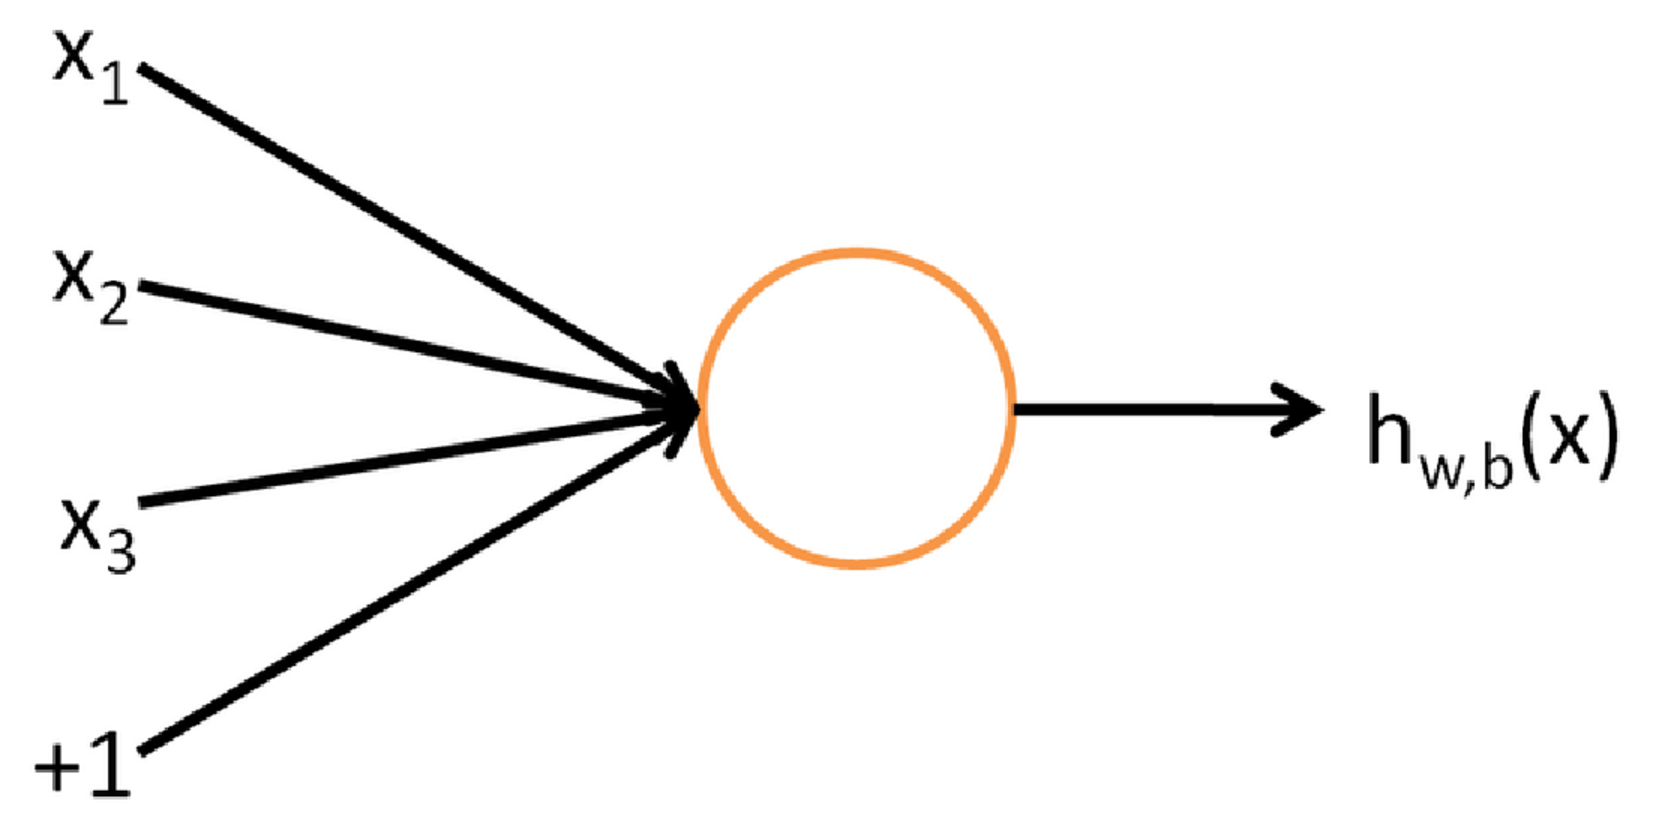
\includegraphics[width=0.5\textwidth]{SingleNeuron}
	\end{figure}
	这个“神经元”是一个以$x_1, x_2, x_3$及截距+1 为输入值的运算单元,其输出为 $h_{W,b}(x) = f(W^Tx) = f(\sum_{i=1}^3 W_{i}x_i +b)$ ,其中函数$f : \Re \mapsto \Re$ 被称为“激活函数”。
	


\end{document}